\documentclass[]{article}

\usepackage[T1]{fontenc}
\usepackage{graphicx}
\usepackage{tabularborder}
\usepackage{booktabs}
\usepackage{tabularx}
\usepackage{float}
\usepackage{tikz}
\usepackage{placeins}
\usepackage{caption}
\usetikzlibrary{shapes}
\usetikzlibrary{fit}
\usepackage{fancyhdr}
\pagestyle{fancy}
\fancyhf{}
\renewcommand{\headrulewidth}{0pt}
\renewcommand{\footrulewidth}{0pt}
\fancyfoot[C]{\thepage}
\usepackage{graphicx}
\usepackage{amsmath}
\usepackage{pgfplots}
\usepackage{float}
\usepackage[margin=1.2in]{geometry}
\usepackage[spanish]{babel}
\usepackage{amsmath}
\usepackage{amssymb}
\usepackage{caption}
\usepackage{subcaption}
\usepackage{graphicx}
\newcommand{\dint}{\delta_{\text{int}}}
\newcommand{\dext}{\delta_{\text{ext}}}
\newcommand{\estado}{(cid,ls,\sigma)}
\newcommand{\R}{\mathbb{R}}
\newcommand{\N}{\mathbb{N}}
\pgfplotsset{compat=1.16}
\title{\textbf{Implementación del Juego de la vida de Conway en PowerDEVS}}
\author{Lucio Mansilla}
\date{\today}

\begin{document}

\maketitle


\section{Introducción / Problema}
El Juego de la Vida de Conway, comúnmente conocido como "Juego de la Vida", es un autómata celular que fue propuesto por el matemático británico John Horton Conway en 1970. Los autómatas celulares son modelos matemáticos para sistemas dinámicos que evolucionan en pasos de tiempo discretos(generaciones). A pesar de su simplicidad aparente, tienen la capacidad de simular sistemas complejos y mostrar comportamientos emergentes, siendo utilizados en diversos contextos, desde la física hasta la teoría de computación.

En el Juego de la Vida, cada celda en una cuadrícula bidimensional puede estar en uno de dos estados: "viva" o "muerta". Las celdas interactúan con sus ocho vecinos adyacentes en horizontal, vertical y diagonal, transicionando entre los estados de vida y muerte de acuerdo a las siguientes reglas de evolución:

\begin{itemize}
\item Cualquier celda viva con dos o tres vecinos vivos sobrevive para la siguiente generación.
\item Cualquier celda viva con menos de dos vecinos vivos muere por soledad para la siguiente generación.
\item Cualquier celda viva con más de tres vecinos vivos muere por superpoblación para la siguiente generación.
\item Cualquier celda muerta con exactamente tres vecinos vivos nace para la siguiente generación.
\end{itemize}

Aunque estas son las reglas originales, existen muchas variantes del Juego de la Vida con diferentes reglas. Además, es posible observar la aparición de diversos patrones, algunos  estáticos, otros oscilan entre varios estados y otros se desplazan por el tablero. Estos patrones serán el objeto de estudio en las secciones posteriores de este informe.

El propósito de este proyecto es explorar la dinámica del juego de una manera visual e interactiva, para ello se implementará el mismo en PowerDEVS, una herramienta de simulación de eventos discretos basada en la teoría DEVS (Discrete Event System Specification).

\section{Especificación DEVS de una celda}

El DEVS que representa únicamente a una célula se define como sigue:

\[ C = \langle X, Y, S, \dint, \dext, \lambda, ta \rangle \]

donde

\begin{itemize}
  \item $X = GameState $

  \item $Y = \N \times \{0,1\}$

  % S = (id, estado, vecinosVivos, vecindarioCambio, proximaAccion, sigma)
  \item $S = \N \times \{0, 1\} \times   \R_0^+$

    El estado es una tupla $(cid, ls, \sigma)$ donde

    \begin{itemize}
      \item $cid \in \N$ es el identificador de la célula.
      \item $ls \in \{0, 1\}$ es el estado de la célula (1 = viva, 0 = muerta)
      \item $\sigma \in \R_0^+$ es el tiempo restante para realizar una próxima salida.
    \end{itemize}

  \item $\dint(\estado) = (cid,ls,\infty)$


  \item $\dext(\estado, e, (x, p)) = \begin{cases}
    (cid,0,1) & ls == 1 \land \not \in SR  \\
    (cid,1,1) & ls == 0 \land \in BR \\
    (cid,ls,1) & \text{otherwise }
  \end{cases}$

    donde $alives = \text{countAlives}(x.rows,x.cols,cid,x.board)$
  \item $\lambda(\estado) = (cid,ls) $
  \item $ta(\estado) = \sigma$

\end{itemize}
    \begin{itemize}
      \item \textbf{countAlives}: La función \textbf{countAlives} tiene como objetivo calcular el número de células vecinas que están vivas para una célula dada. Esta función recibe cuatro parámetros: el número de filas (rows) y columnas (cols) del tablero, el identificador de la célula (cell\_id) y el estado actual del tablero (board). La función opera de la siguiente manera:

        \item Primero, determina la ubicación (fila y columna) de la célula dada en el tablero usando su identificador (cell\_id) y las dimensiones del tablero.
        \item Posteriormente, recorre todas las células vecinas de la célula dada. Esto se realiza iterando a través de todas las posibles combinaciones de desplazamientos en filas y columnas en el rango de -1 a 1. 
        \item Ignora la propia célula durante la iteración, es decir, el caso cuando tanto el desplazamiento de la fila como de la columna es cero.
        \item Para cada célula vecina, primero verifica si está dentro de los límites del tablero. Si la célula vecina está fuera de los límites del tablero, pasa a la siguiente iteración.
        \item Si la célula vecina está dentro de los límites, verifica si está viva, es decir, si su estado en el tablero es 1. Si es así, incrementa un contador de células vivas.
        \item Finalmente, después de haber iterado a través de todas las células vecinas, la función devuelve el contador de células vivas.
    \end{itemize}




% Aquí puedes detallar cómo especificaste una celda del juego en DEV
\section{Implementación en PowerDEVS}
% En esta sección puedes describir los patrones que has implementado.
\section{Patrones}
El Juego de la Vida, concebido por el matemático británico John Horton Conway, es famoso por la vasta variedad de patrones que emergen de sus simples reglas, en particular, las reglas 23/3. Los patrones se definen como configuraciones de células que se repiten tras un número determinado de generaciones, también conocido como su "periodo". Los patrones pueden ser estáticos, oscilantes o móviles, dependiendo de cómo cambian a lo largo del tiempo. En las secciones siguientes se presentarán ejemplos de estos patrones bajo las reglas 23/3.

\subsection{Patrones estáticos}
Los patrones estáticos, también conocidos como "still lifes", son configuraciones de células que no cambian de una generación a la siguiente, es decir, su periodo es 1. A continuación, se presentan ejemplos de estos patrones:

\begin{figure}[H]
  \centering
  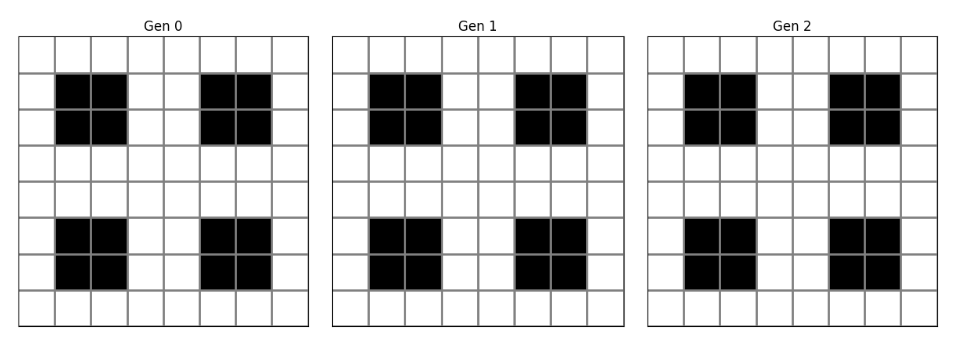
\includegraphics[width=0.75\textwidth]{../assets/still_life/block/block.png}
  \caption{Patrón bloque: un patrón estático compuesto por un cuadrado de 2x2 células. Aparece frecuentemente debido a su simplicidad.}
  \label{fig:block}
  \end{figure}

\begin{figure}[H]
  \centering
  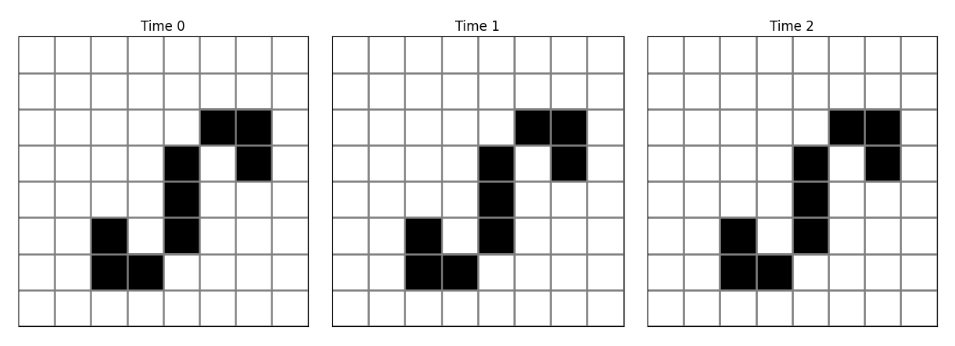
\includegraphics[width=0.75\textwidth]{../assets/still_life/integral/integral.png}
  \caption{Patrón integral: este patrón estático se asemeja a la forma de un signo integral.}
  \label{fig:integral}
  \end{figure}

\begin{figure}[H]
  \centering
  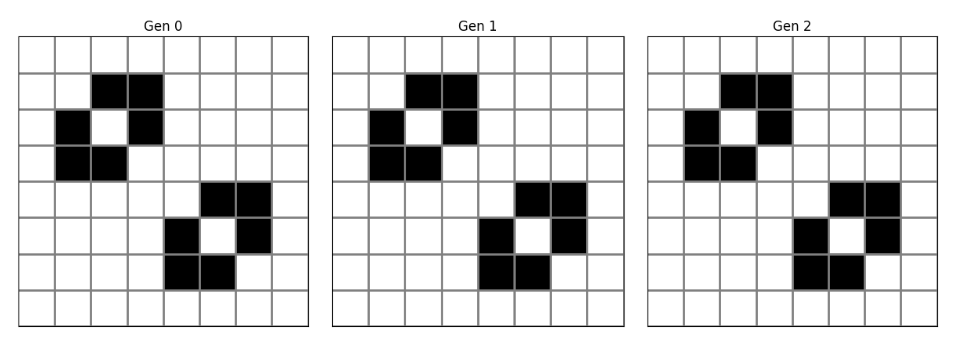
\includegraphics[width=0.75\textwidth]{../assets/still_life/ship/ship.png}
  \caption{Patrón ship: este patrón estático se asemeja a la forma de una nave espacial.}
  \label{fig:ship}
  \end{figure}

\begin{figure}[H]
  \centering
  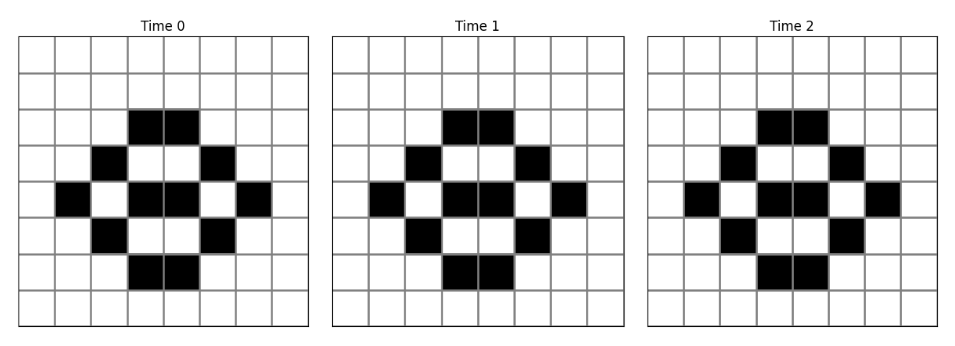
\includegraphics[width=0.75\textwidth]{../assets/still_life/honeycomb/honeycomb.png}
  \caption{Patrón honeycomb: este patrón estático se asemeja a la estructura de un panal de abejas.}
  \label{fig:honeycomb}
  \end{figure}

\subsection{Osciladores}
Los osciladores son patrones que vuelven a su configuración inicial después de un número fijo de generaciones, llamado su período. A diferencia de los patrones estáticos, los osciladores cambian su apariencia durante su ciclo de vida, pero eventualmente vuelven a su estado original. Un ejemplo famoso de oscilador es el "blinker", que oscila entre una orientación horizontal y vertical cada generación.

\begin{figure}[H]
  \centering
  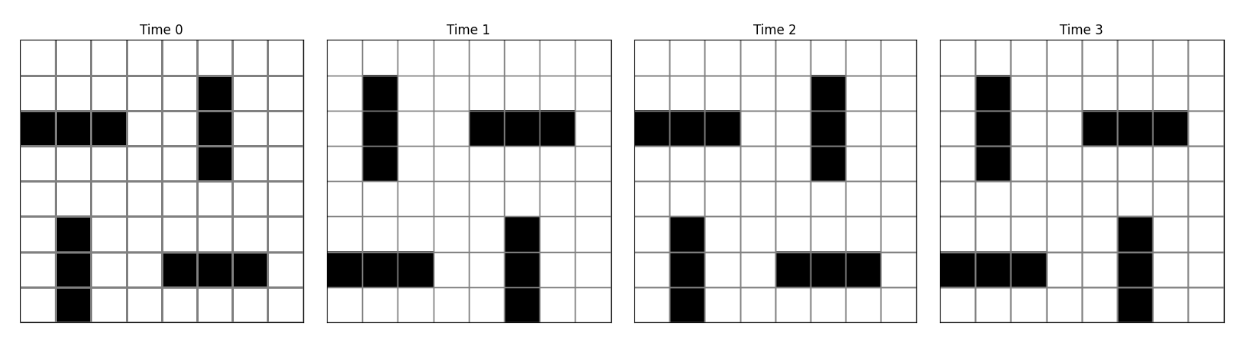
\includegraphics[width=0.9\textwidth]{../assets/oscillator/blinker/blinker.png}
  \caption{Patrón blinker: un oscilador de periodo 2. Oscila entre una orientación horizontal y vertical cada generación. Notar que en este caso hay 4 blinkers en el tablero.}
  \label{fig:blinker}
  \end{figure}

  \begin{figure}[H]
    \centering
    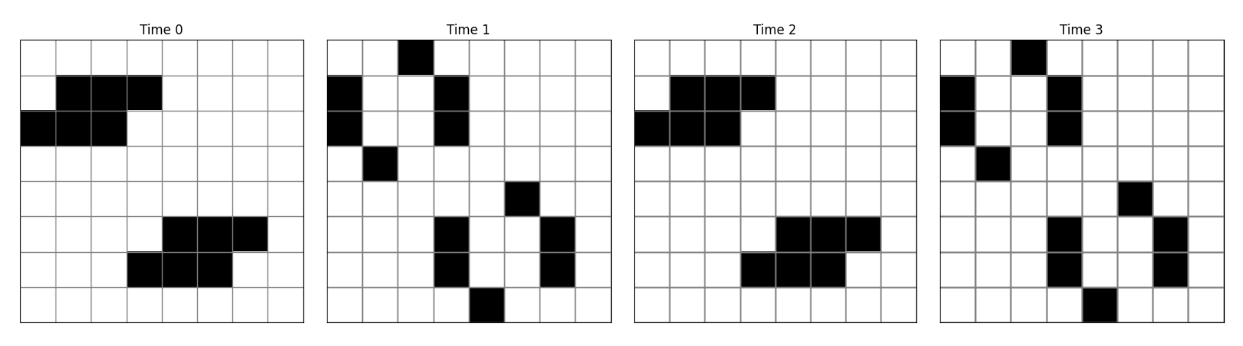
\includegraphics[width=0.9\textwidth]{../assets/oscillator/toad/toad.png}
    \caption{Patrón toad: }
    \label{fig:toad}
    \end{figure}

    \begin{figure}[H]
      \centering
      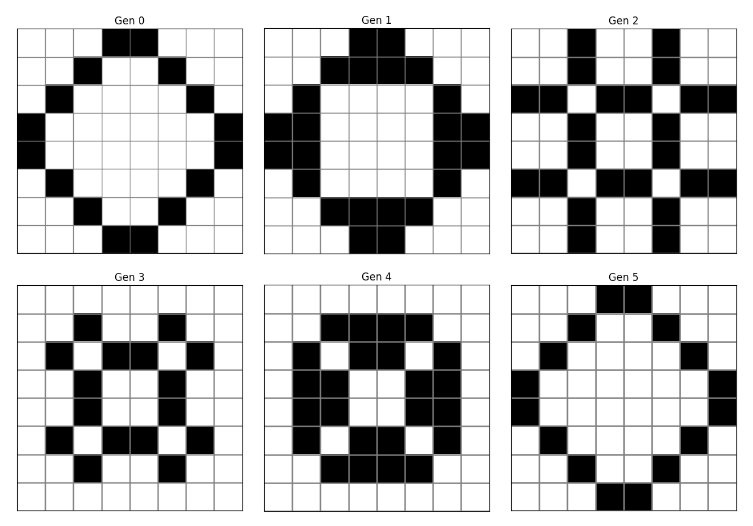
\includegraphics[width=0.7\textwidth]{../assets/oscillator/octagon_2/octagon_2.png}
      \caption{Patrón octagon: }
      \label{fig:octagon}
      \end{figure}
% Aquí puedes insertar una figura de un blinker u otro oscilador.

\subsection{Naves espaciales}
Las naves espaciales son patrones que se trasladan a través de la cuadrícula mientras oscilan. El ejemplo más conocido es la "nave ligera" (o "glider" en inglés), que se desplaza diagonalmente a través de la cuadrícula mientras oscila entre cuatro configuraciones diferentes.

\subsection{Methuselahs}
Los Methuselahs son patrones que evolucionan durante un número grande de generaciones antes de estabilizarse en un patrón estático, un oscilador o una nave espacial. El ejemplo más conocido es el "acorn", que evoluciona durante 5206 generaciones antes de estabilizarse en 633 células vivas, incluyendo 11 osciladores, 2 naves espaciales y 1 patrón estático.

% Aquí puedes insertar una figura de una nave ligera u otra nave espacial.

\subsection{Patrones Propios}
Sección dedicada a patrones que encontramos por accidente/pruebas.

\subsection{Patrones complejos}
Además de estos patrones simples, también existen patrones más complejos en el Juego de la Vida. Algunos de estos pueden "disparar" naves espaciales, otros pueden "construir" patrones adicionales, y otros pueden incluso comportarse como máquinas de Turing universales, lo que significa que pueden computar cualquier función computable.

% Aquí puedes insertar figuras de patrones complejos y discutir sus propiedades.

Estos patrones ilustran la increíble diversidad de comportamientos que pueden surgir del Juego de la Vida. En las siguientes secciones, veremos cómo estos patrones pueden ser generados e investigados usando PowerDEVS.



\section{Conclusiones}
\end{document}
